\documentclass[12pt,a4paper,openany]{memoir}
\usepackage[utf8]{inputenc}
\usepackage[T1]{fontenc}
\usepackage{microtype}
\usepackage[dvips]{graphicx}
\usepackage{xcolor}
\usepackage{times}
\usepackage[french]{babel}
\usepackage[export]{adjustbox}
\usepackage{subcaption}

\usepackage[
breaklinks=true,colorlinks=true,
%linkcolor=blue,urlcolor=blue,citecolor=blue,% PDF VIEW
linkcolor=black,urlcolor=black,citecolor=black,% PRINT
bookmarks=true,bookmarksopenlevel=2]{hyperref}

\usepackage{geometry}
\usepackage{float}
\usepackage{listings}
\usepackage{color}

\definecolor{codegreen}{rgb}{0,0.6,0}
\definecolor{codegray}{rgb}{0.5,0.5,0.5}
\definecolor{codepurple}{rgb}{0.58,0,0.82}
\definecolor{backcolour}{rgb}{0.95,0.95,0.92}
 

\lstdefinelanguage{JavaScript}{
  keywords={typeof, new, true, false, catch, function, return, null, catch, switch, var, if, in, while, do, else, case, break},
  keywordstyle=\color{blue}\bfseries,
  ndkeywords={class, export, boolean, throw, implements, import, this},
  ndkeywordstyle=\color{darkgray}\bfseries,
  identifierstyle=\color{black},
  sensitive=false,
  comment=[l]{//},
  morecomment=[s]{/*}{*/},
  commentstyle=\color{purple}\ttfamily,
  stringstyle=\color{red}\ttfamily,
  morestring=[b]',
  morestring=[b]"
}
 
\lstdefinestyle{mystyle}{
    backgroundcolor=\color{backcolour},   
    commentstyle=\color{codegreen},
    keywordstyle=\color{magenta},
    numberstyle=\tiny\color{codegray},
    stringstyle=\color{codepurple},
    basicstyle=\footnotesize,
    breakatwhitespace=false,         
    breaklines=true,                 
    captionpos=b,                    
    keepspaces=true,                 
    numbers=left,                    
    numbersep=5pt,                  
    showspaces=false,                
    showstringspaces=false,
    showtabs=false,                  
    tabsize=2
}
 
\lstset{style=mystyle}

% PDF VIEW
% \geometry{total={210mm,297mm},
% left=25mm,right=25mm,%
% bindingoffset=0mm, top=25mm,bottom=25mm}
% PRINT
\geometry{total={210mm,297mm},
left=20mm,right=20mm,
bindingoffset=10mm, top=25mm,bottom=25mm}

\OnehalfSpacing
%\linespread{1.3}

%%% CHAPTER'S STYLE
%\chapterstyle{bianchi}
%\chapterstyle{ger}
\chapterstyle{madsen}
%\chapterstyle{ell}
%%% STYLE OF SECTIONS, SUBSECTIONS, AND SUBSUBSECTIONS
\setsecheadstyle{\Large\bfseries\sffamily\raggedright}
\setsubsecheadstyle{\large\bfseries\sffamily\raggedright}
\setsubsubsecheadstyle{\bfseries\sffamily\raggedright}


%%% STYLE OF PAGES NUMBERING
%\pagestyle{companion}\nouppercaseheads 
%\pagestyle{headings}
%\pagestyle{Ruled}
\pagestyle{plain}
\makepagestyle{plain}
\makeevenfoot{plain}{\thepage}{}{}
\makeoddfoot{plain}{}{}{\thepage}
\makeevenhead{plain}{}{}{}
\makeoddhead{plain}{}{}{}


\maxsecnumdepth{subsection} % chapters, sections, and subsections are numbered
\maxtocdepth{subsection} % chapters, sections, and subsections are in the Table of Contents


%%%---%%%---%%%---%%%---%%%---%%%---%%%---%%%---%%%---%%%---%%%---%%%---%%%

\begin{document}

%%%---%%%---%%%---%%%---%%%---%%%---%%%---%%%---%%%---%%%---%%%---%%%---%%%
%   TITLEPAGE
%
%   due to variety of titlepage schemes it is probably better to make titlepage manually
%
%%%---%%%---%%%---%%%---%%%---%%%---%%%---%%%---%%%---%%%---%%%---%%%---%%%
\thispagestyle{empty}
{
	\sffamily
	\centering
	\large

	~\vspace{\fill}

	{\huge Rapport TERL - Réalisation d’un outil de gestion de l’emploi du temps}


	\vspace{2.5cm}

	\begin{itemize}
	    \item BOURGIN Jérémy
	    \item MANSOURI Hind
	    \item RAIHAUTI Teiki
	    \item TERKI Adel
	\end{itemize}

	\vspace{2.5cm}

	Université de Montpellier 
	
	\vspace{2.5cm}
	
	
\includegraphics{img/logo.png}

	\vspace{2.5cm}

	Encadrante : Mme BOUZIANE Hinde

	\vspace{\fill}

	Mai 2017
}

\clearpage
\tableofcontents
\clearpage

%%%---%%%---%%%---%%%---%%%---%%%---%%%---%%%---%%%---%%%---%%%---%%%---%%%
%%%---%%%---%%%---%%%---%%%---%%%---%%%---%%%---%%%---%%%---%%%---%%%---%%%

\chapter{Introduction}
\par
Tout d'abord nous souhaitons remercier Mme BOUZIANE Hinde notre encadrante de projet pour son soutien et les efforts fournis dans l'avancée de ceui-ci.
\par
Dans le cadre du projet de deuxième année de licence informatique, nous devions réaliser un générateur d'emploi du temps destiné aux enseignants du département informatique de la Faculté des Sciences de Montpellier.
\par
Nous avons décidé d'implémenter un algorithme de génération d'emploi du temps respectant de multiples contraintes et de mettre en place une application internet pour gérer l'emploi du temps en question.
\par
Après avoir structuré l'ensemble du travail à réaliser, nous avons pu répartir les tâches pour optimiser notre temps de travail. Pour cela, nous avons divisé le projet en 2 points : 
\begin{itemize}
    \item Conception et implémentation du générateur d'emploi du temps.
    \item Les fonctionnalités de notre application web.
\end{itemize}
\par
Nous sommes un groupe de quatre personnes alors la répartition des tâches s'est faite naturellement : deux personnes sur la réalisation du générateur d'emploi du temps, et deux personnes sur les fonctionnalités de la plateforme. Pour un bon partage du travail de chacun, nous avons utilisé le GitLab de l'Université. De plus, cela nous a permis d'avancer le projet en-dehors de l'université sans conflits.
\par
Quant à la rédaction du rapport, nous avons utilisé le site ShareLatex pour les mêmes raisons que citées précédemment.

\chapter{Conception}
\section{Les différentes problématiques}
\par
La conception d'un emploi du temps est basée sur un ensemble de paramètres. Dans le cadre de notre projet, ce sont des contraintes. Cependant, créer un emploi du temps manuellement est problématique car il y a un nombre important de contraintes. Il faut aussi que toutes les séances soient disposées de manière cohérente. Ainsi, nous allons voir que concevoir un outil est efficace. Pour cela, nous nous sommes appuyé sur les points suivants :
\begin{itemize}
    \item Réaliser un outil permettant de créer un emploi du temps à partir de multiples contraintes. 
    \item Définir et modéliser les différentes contraintes.
    \item Implémenter l'outil.
\end{itemize}

\section{Les fonctionnalités :}
\par
Pour répondre aux besoins du projet, il fallait implémenter les fonctionnalités suivantes de façon à permettre aux responsable d'UE :
\begin{itemize}
	\item De saisir leurs indisponibilités.
	\item D'indiquer des créneaux de préférences.
	\item D'indiquer quand des séances doivent se succéder.
\end{itemize}
\par
Et permettre aux responsables de promotion :
\begin{itemize}
	\item De saisir des créneaux non disponibles à la réservation pour une promotion ou un groupe (exemples des créneaux dédiés à des UE CMI). 
	\item D'indiquer pour une promotion si elle peut faire une journée 8h/20h, complète ou non.
	\item Garantir les pauses déjeuner.
\end{itemize}
% finir la section %
\clearpage

\section{Collecte des contraintes}
\par
Nous appelons contraintes :
    \begin{itemize}
    \item Tous les créneaux durant lesquels une séance ne peut pas avoir lieu
    \item Les séances qui doivent se succéder
    \item Les pauses déjeuner et empêcher les journées de 8h/20h 
    \end{itemize}
Pour collecter les différentes contraintes, nous avons mis l'accent sur des fonctionnalités intuitives et accessibles aux utilisateurs. De cela découle deux points fondamentaux pour notre application :
\begin{itemize}
	\item Donner un format paramétrable et utilisable pour la génération de l'emploi du temps.
	\item Définir une interface simple et ergonomique pour chaque fonctionnalité.
\end{itemize}
\par
À partir de ce moment là, nous avons pu définir toutes les fonctionnalités nécessaires aux besoins du projet et nous en avons conçu trois : 
\begin{itemize}
	\item Ajouter des contraintes et préférences en cochant des cases dans un emploi du temps (voir l'annexe). Chaque case cochée est représentée par un jour et une heure au format numérique.
	\item Pour permettre aux enseignants d'indiquer que des séances doivent se succéder, nous avons mis en place un système que nous avons appelé groupement (puisque le principe est de regrouper des séances).
	Ce système permet d'enchaîner des séances dans l'ordre séance mère -> séance fille.
	\item Pour empêcher à une promotion de faire une journée complète 8h/20h et garantir les pauses déjeuner, nous avons imaginé un système que nous avons nommé complétion.
	Une complétion a besoin de 2 heures différents pour fonctionner, appelons les heure A et heure B. Lorsque une séance est planifiée commençant à l'heure A, alors le créneau de l'heure B devra rester libre pour les étudiants et vice-versa.
\end{itemize} 

\section{Résolution des contraintes}
\par
Pour résoudre les contraintes et avoir un emploi du temps cohérent, nous avons créé un algorithme qui place les séances une par une. Il recherche les créneaux libres où l'on peut placer la séance. De là, deux cas de figure s'ouvrent à nous :
\begin{itemize}
    \item S'il y a des créneaux libres, le programme place la séance au premier créneau trouvé
    \item S'il n'y en a pas, la séance du premier créneau respectant les contraintes sera déplacée suivant le même procédé, c'est à dire : recherche des créneaux libres et déplacement des séances gênantes.
\end{itemize}
\par
Mais une image vaut mille mots alors les schémas ci-dessous permettent d'illustrer le déroulement général de l'algorithme. Pour simplifier la compréhension, nous illustrons le principe de notre solution sur 4 séances placées sur une journée. Les séances sont caractérisées par leurs noms (S1.. S4) et par les groupes participant à la séance (A, B, A et B).

\clearpage
Voici les contraintes des quatre séances :

\begin{figure}[H]
   \begin{minipage}{0.4\linewidth}
      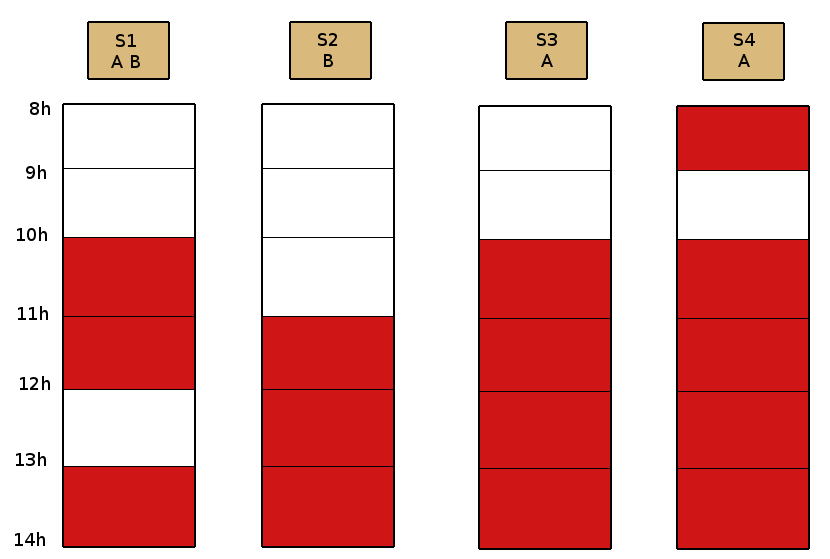
\includegraphics[scale=0.22]{img/Schema/Contrainte.png}
      \caption{Contraintes}
   \end{minipage} \hfill
   \begin{minipage}[c]{0.5\linewidth}
    Ce schéma définit un exemple de 4 séances avec des contraintes sur une journée. Les séances sont en dorées et chaque case du tableau représente un créneau du lundi. Les cases rouges sont les contraintes.
   \end{minipage}
\end{figure}

\begin{figure}[H]
    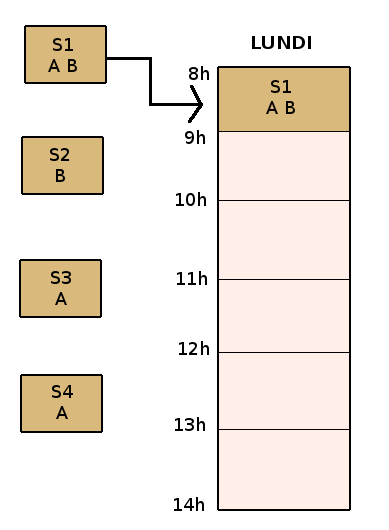
\includegraphics[scale=0.3]{img/Schema/Etape_1.png} \hfill
    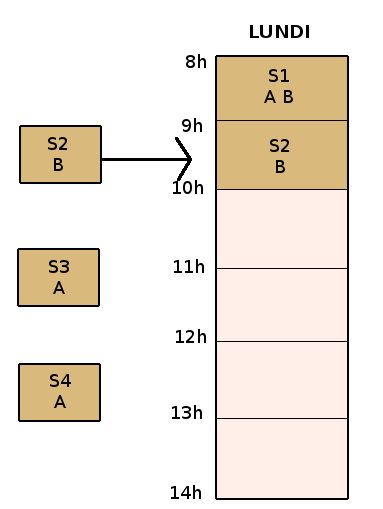
\includegraphics[scale=0.3]{img/Schema/Etape_2.png}
    \caption{Placement de S1 et S2} \medbreak
    \par La première séance est placée dans la première case libre de l'emploi du temps respectant les contraintes. Ici, S1 est placée au créneau de 8h-9h.
    \par Ensuite, S2 est placée à 9h car en effet, la séance de 8h la bloque. 
\end{figure}

\begin{figure}[H]
   \begin{minipage}{0.35\linewidth}
      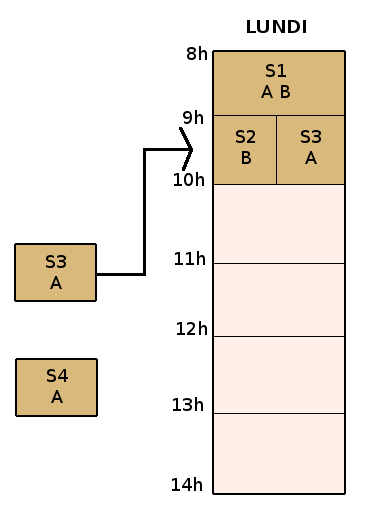
\includegraphics[scale=0.3]{img/Schema/Etape_3.png}
      \caption{Placement de S3}
   \end{minipage} \hfill
   \begin{minipage}[c]{0.64\linewidth}
    S3 ne va pas se placer à 10h car le créneau de 9h ne concerne que le groupe B. Or S3 est un cours du groupe A et il est donc possible de placer S3 sur le même créneau que S2.
   \end{minipage}
\end{figure}

\begin{figure}[H]
    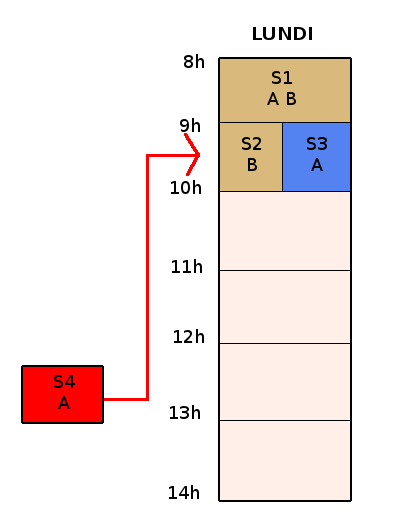
\includegraphics[scale=0.3]{img/Schema/Etape_4.png}\hfill
    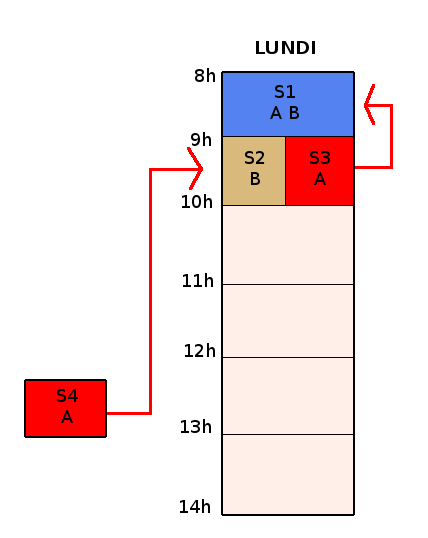
\includegraphics[scale=0.3]{img/Schema/Etape_5.png}
    \caption{Placement de S4} \medbreak
    \par Le seul créneau possible pour S4 est celui de 9h, il est donc indispensable de déplacer les cours gênants. S4 n'étant un cours ne concernant que le groupe A, seul S3 va être déplacé.
    \par Le seul créneau où S3 peut se placer est celui de 8h. Nous allons donc appliquer le même procédé à S1 et lui chercher un nouveau créneau.
\end{figure}

\begin{figure}[H]
    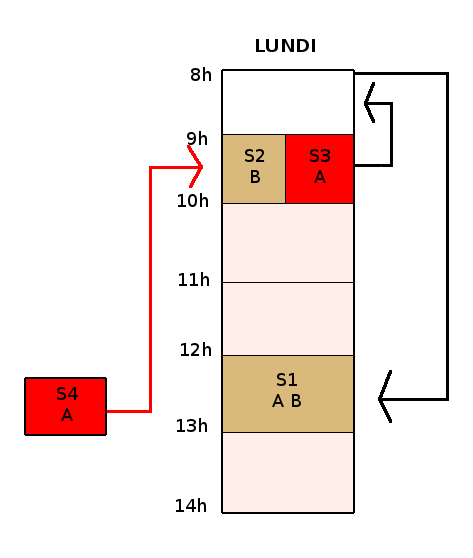
\includegraphics[scale=0.3]{img/Schema/Etape_6.png}\hfill
    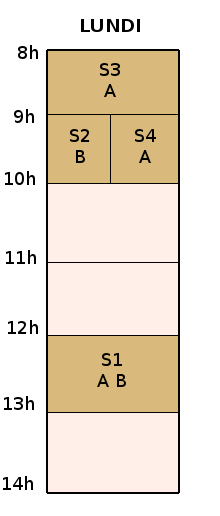
\includegraphics[scale=0.3]{img/Schema/Etape_7.png}
    \caption{Derniers déplacements} \medbreak
    \par S1 a pu être placé sans encombre au créneau de 15h, ce qui va libérer de l'espace pour S3 et par la même occasion, pour S4.
    \par L'algorithme a permis de placer toutes les séances du lundi pour une promo donnée.
\end{figure}
\clearpage


\subsection{Les contraintes et préférences}
\par 
Puisqu'il est possible d'attribuer des contraintes à des promotions, groupes, UE et séances, il faut rassembler les contraintes pour faciliter leurs gestions. Pour cela, nous allons les affecter uniquement dans les séances concernées. \par
Nous vérifions pour chaque séance, les créneaux dans lesquels elle pourrait être placée. Ainsi est rassemblée la totalité des cellules respectant les contraintes dans un tableau. \par
Ce système permet de placer au maximum les préférences, en effet il suffit de mettre les cellules respectant les préférences au début de ce tableau.

\subsection{Les groupements (enchaînement de séances)}
\par
Les groupements de séances sont présentées sous forme d'une liste doublement chaînée. Les séances sont alors dépendantes les unes des autres. Par conséquent, filtrer l'ensemble des séances pour ne garder que les séances racine (le premier élément de la liste) est une étape primordiale.
\par
Afin de respecter les groupements, l'algorithme de résolution de contraintes se charge de chercher des cellules libres en fonction de toute la liste, et renvoyer uniquement les cellules convenantes à la séance racine. Enfin, lorsque une séance sera placée dans une cellule, les séances filles se placeront naturellement dans les cellules qui suivent.

\subsection{Les complétions (séances virtuelles)}
\par
En utilisant le principe des complétions, dès qu'une séance est placée à l'heure A alors une séance virtuelle reliée est placée à l'heure B indiquée. La particularité est que la séance virtuelle va empêcher le placement d'une véritable séance et par conséquent, va laisser un créneau de libre. Grâce à ce système, nous allons pouvoir répondre à 2 besoins dans le projet : 
\begin{itemize}
    \item Garantir les pauses déjeuner, car il suffit de créer une complétion qui a pour heure A 11h30 et pour heure B 13h15.
    \item Éviter les journées complètes 8h - 20h en créant une complétion qui a pour heure A 8h et pour heure B 18h30.
\end{itemize}
\par
De plus, dans l'optique de limiter les journées chargées, ce système garantit plus de souplesse. Par exemple il est possible de limiter une journée à 8h/16h30 ou 9h30/18h.

\section{Architecture de l'outil}
\par
Nous avons décidé de réaliser des diagrammes UML, car cela permet de conceptualiser un projet, représenter les données et leurs structures. Ainsi, cela permet une meilleure cohésion au sein d'un groupe, et d'éviter tout mal entendu avec le client. \par
Pour commencer, nous avons décidé de réaliser un diagramme entité-relation afin de représenter les entités nécessaire à l'algorithme de résolution de contraintes : 
\begin{figure}[H]
    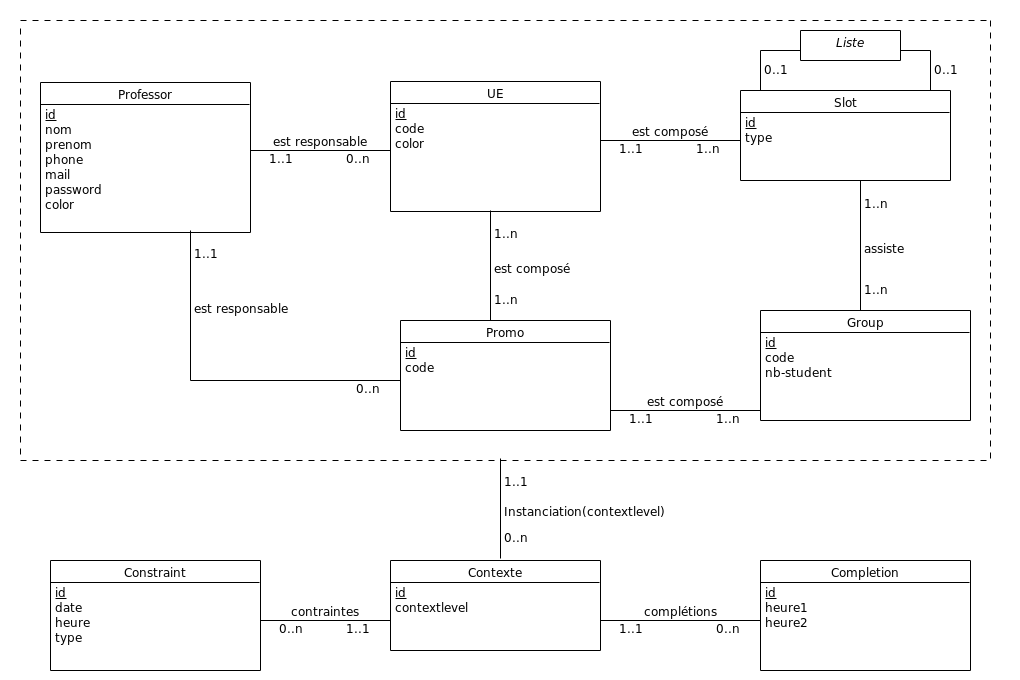
\includegraphics[width=19cm, center]{img/BDD_edt.png}
    \caption{Diagramme entité-relation}
\end{figure}
\par
D'après le modèle ci dessus on peut aussi déduire que : 
\begin{itemize}
    \item Un professeur peut être responsable de plusieurs UE et promotions.
    \item Une promotion est composée de plusieurs groupes.
    \item Un ou plusieurs groupes peuvent assister à une ou plusieurs séances.
    \item Une UE est composée de plusieurs séances.
    \item Une séance peut être composée de plusieurs autres séances (cas de succession de séances).
\end{itemize}
\medbreak

L'entité Contexte est particulière. En effet, elle peut être liée à un professeur, une promo, une UE, une séance ou un groupe. Cela permet de placer des contraintes sur toutes ces entités grâce à une clé étrangère et un attribut contextlevel défini comme suit : 
\begin{itemize}
    \item contextlevel = 1 -> Promo
    \item contextlevel = 2 -> Group
    \item contextlevel = 3 -> Professor
    \item contextlevel = 4 -> UE
    \item contextlevel = 5 -> Slot
\end{itemize}
\bigbreak
\par
Nous allons maintenant voir le diagramme de classe qui est la suite logique du diagramme précédent :
\begin{figure}[H]
    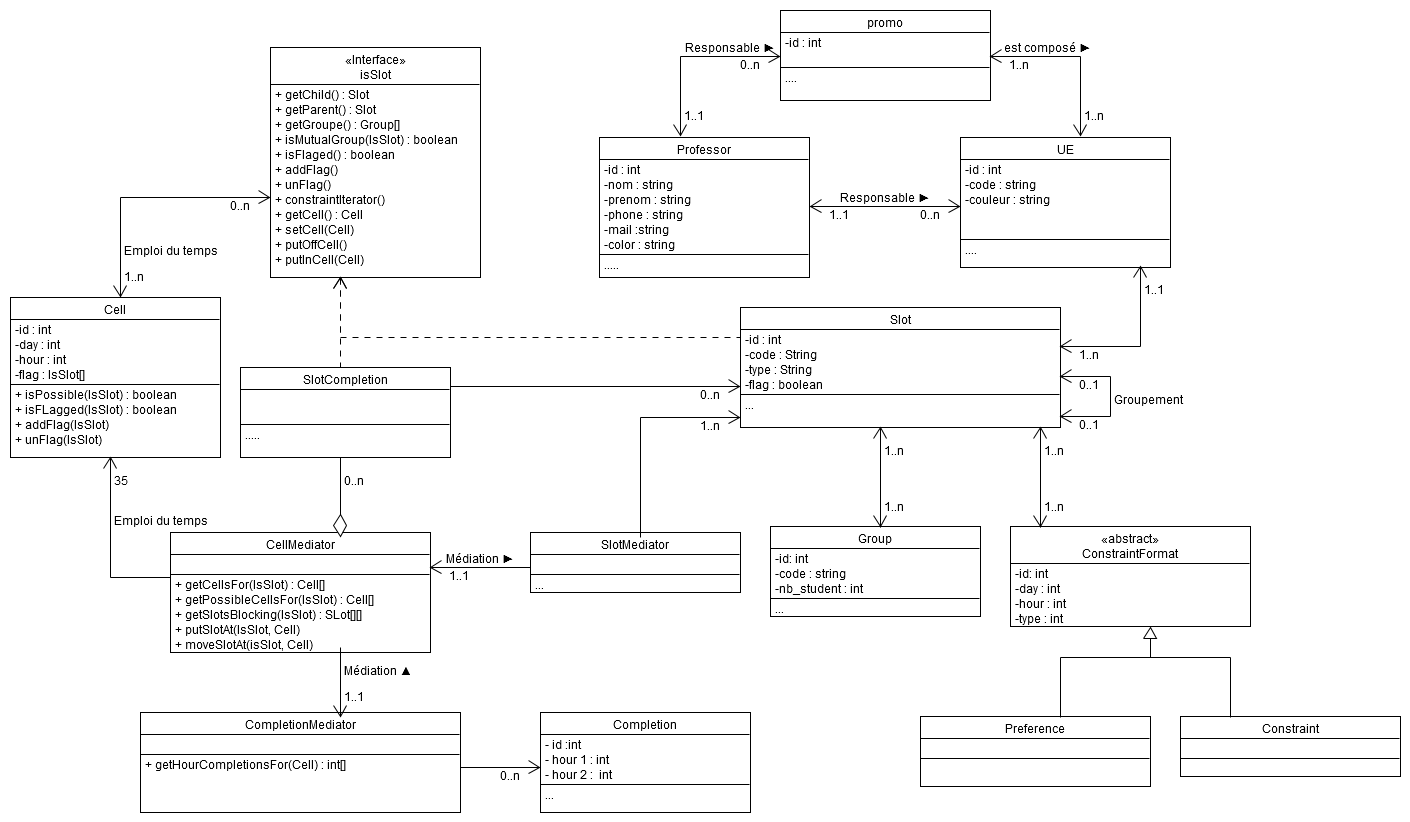
\includegraphics[width=20cm, center]{img/UML_class.png}
    \caption{Diagramme de classe}
\end{figure}
\par
Le but de ce diagramme est de respecter au mieux notre algorithme de résolution de contraintes. Par exemple, nous savons qu'une cellule peut contenir plusieurs séances à condition que celles-ci ne possèdent pas de groupe en commun. \par 
Pour faciliter la communication entre les instances des classes Completion, Cell et Slot, il y les services SlotMediator, CellMediator et CompletionMediator. Par exemple, CompletionMediator sera sollicitée afin de fournir un tableau d'heures pour lesquelles des séances de complétions seront insérées.

\clearpage

\chapter{Implémentation}
\section{Les choix techniques}
\par
Dans le cadre d'un projet, les choix techniques doivent dépendre de l'environnement de celui-ci. Dans notre cas, nous avons réalisé une plateforme web qui permet à un utilisateur de saisir les données utiles à la génération d'un emploi du temps. Cependant l'algorithme doit pouvoir fonctionner pleinement sans l'application.
Nous avons préféré faire de la plateforme web l'élément central de notre projet. Cela permet, par exemple, la distribution d'un logiciel, l'authentification, les connexions aux bases de données...
\medbreak
\par
Le langage PHP nous a paru comme un langage optimal pour notre générateur car il a été spécialement conçu pour le web, il est très bien documenté et nous pouvons utiliser le paradigme d'objet. Il est implémenté sur le serveur web local de l'université.
\par
Aussi, nous avons décidé d'utiliser une base de données MySQL. Elle nous permet de stocker, récupérer et représenter des données très facilement sachant qu'il y a un module intégré à PHP.
\par
Puisqu'il était essentiel pour nous d'utiliser le plus possible la programmation orientée objet, un ORM (mapping objet-relationnel) était indispensable. Néanmoins, nous avons eu besoin d'un système simple et performant. C'est pourquoi, au vu de la complexité des outils comme Doctrine, nous avons décidé de concevoir notre propre ORM, adapté pour modéliser nos données.
\medbreak
\par
Enfin, pour le développement de la plateforme web côté client, il est incontournable d'utiliser le HTML, le CSS, et le Javascript. Cependant, pour des soucis d'ergonomie et de rapidité, nous avons privilégié au maximum l'utilisation de Javascript en utilisant l'Ajax et le JSON. Ainsi, cela évite d'utiliser un système de template côté client, souvent lourd pour un serveur. La génération de l'emploi du temps peut demander une charge importante de travail au serveur, il était donc important de limiter au maximum ces charges. C'est pour cela que nous avons décidé d'utiliser AngularJS, qui permet de gérer plus facilement un environnement comme celui-ci.

\clearpage

\section{Solutions techniques}
\par 
Devant la panoplie d'outils cités précédemment, il fallait faire les bon choix et optimiser au maximum leur utilisation. Pour cela, AngularJS et l'ORM ont été 2 points clé à notre projet.
\subsection{AngularJS}
AngularJS est un framework Javascript suivant le patron de conception MVC (Modèle Vue Controller), très utilisé dans le dévelopement web. Il permet d'étendre l'utilisation du langage Javascript.
\par
Les contrôleurs sont des modules d'AngularJS permettant l'interaction et l'échange de données entre le HTML (la vue) et le javascript (Modèles/Données). Le framework permet d'utiliser simplement ce principe de la façon suivante :
\begin{lstlisting}[language=JavaScript]
var app = angular.module('ue', []);
app.controller('constraintController', constraintController);
constraintController.$inject = ['$scope', 'MonFactory'];

function constraintController($scope, MonFactory) {
	.......
}

\end{lstlisting}
\par
Puis grâce aux directives d'AngularJs, il suffit de lier notre contrôleur au HTML de cette façon :
\begin{lstlisting}
<body ng-app="ue">
...
<section ng-controller="constraintController">
    ...
</section>
...
</body>
\end{lstlisting}
\par 
Enfin, pour interagir entre le JavaScript et le HTML (la vue), il suffit simplement d'intégrer des éléments du code dans ce qui est appelé le scope :
\begin{itemize}
    \item Dans le javascript :
     \begin{lstlisting}[language=JavaScript]
        var monNom = "...";
        $scope.name = monNom;
    \end{lstlisting}
    \item Dans le HTML :
    \begin{lstlisting}[language=JavaScript]
        {{name}}
    \end{lstlisting}
\end{itemize}

\par 
Les contrôleurs étant indépendant les uns des autres, il était important de créer ce que l'on appelle des factory. Cela nous a permit de centraliser des parties du code afin de ne pas se répéter entre les différents contrôleurs. La création et l'utilisation d'un factory reste elle aussi simple :
\begin{lstlisting}[language=JavaScript]
angular.module('ue').factory('MonFactory',MonFactory);
MonFactory.$inject = [];

function MonFactory() {
    return {
        f1 : f1,
        ....
    };

    .....//les fonctions et variables du service 
    function f1(){
        ....
    }
}
\end{lstlisting}
\par 
Enfin, on injecte le service dans le contrôleur désiré pour utiliser les fonctions de ce dernier, comme ceci :
\begin{lstlisting}[language=JavaScript]
MonControlleur.$inject=['MonFactory'];
\end{lstlisting}

\subsection{PHP}
\par
Pour pouvoir modéliser les données de la base de données sous forme d'objets, nous utilisons une technique appelée l'ORM qui consiste à transformer un tableau associatif (résultat d'une requête SQL) en un objet.
\par
Tout d'abord avec la méthode \textit{getConnexion()} nous pouvons nous connecter à la base de données désirée, implémenter la requête SQL avec la méthode \textit{createQuery("MaRequêteSQL")} puis l'exécuter. Grâce à la méthode \textit{query()} l'objet contenant les résultats de la requête SQL peut être récupéré et enfin avec \textit{ORM::modelise(\$obj,"MaClasse")} on récupère un tableau d'objets à partir de la classe indiquée.
L'utilisation de cette technique se fait à travers ces lignes de codes :
\begin{lstlisting}[language=PHP]
$pdo = SGBD::getConnexion();
$sql = $pdo->createQuery("SQL");
$query = $sql->query();
$result = ORM::modelise($query,"MaClasse");
\end{lstlisting}

\section{Interface graphique}
\par
L'interface graphique est un point important dans l'implémentation des fonctionnalités. Le design doit être soigné et doit respecter certaines règles d'ergonomie primordiale (par exemple la règle des 3 clics). La section portera sur la conception et l'utilisation de notre plateforme.
\par
\subsection{Les contraintes}
\begin{figure}[H]
    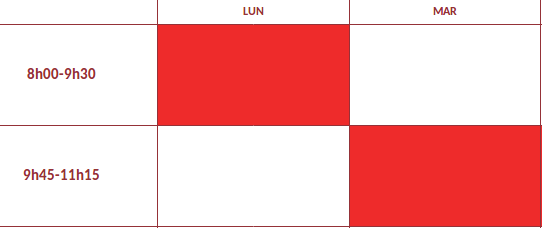
\includegraphics[scale=0.3]{img/interfaces/contrainte.png}\hfill
    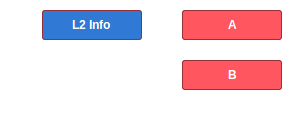
\includegraphics[scale=0.3]{img/interfaces/contrainte_promo.png}\hfill
    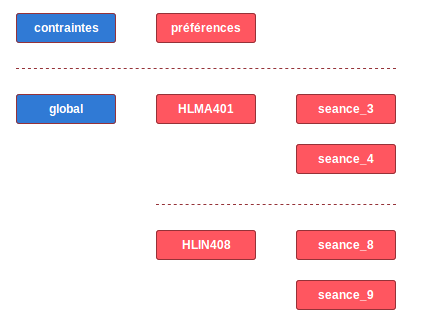
\includegraphics[scale=0.3]{img/interfaces/contrainte_ue.png}
    \caption{Saisie des contraintes} \medbreak
\end{figure}
\par
Des contraintes peuvent être saisies pour des entités telles qu'une promotion, un groupe, une UE ou une séance. Pour cela, il suffit simplement de sélectionner (case en bleu) l'entité souhaitée (image du milieu et de droite). Pour saisir les contraintes, il suffit de cliquer sur les cases dans l'emploi du temps dont on souhaite indiquer une indisponibilité (image de gauche). Les préférences sont saisies de la même façon.

\subsection{Les groupements}
\begin{figure}[H]
   \begin{minipage}{0.3\linewidth}
      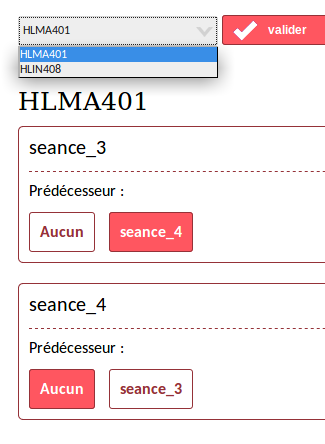
\includegraphics[scale=0.4]{img/interfaces/groupement.png}
      \caption{Enchaîner les cours}
   \end{minipage} \hfill
   \begin{minipage}[c]{0.65\linewidth}
    Nous avons décidé de regrouper les séances par UE. Ainsi cela évite que les séances soient mélangées. \\
    Enfin, pour saisir un groupement, il suffit d'indiquer les prédécesseurs de chaque séance. 
   \end{minipage}
\end{figure}

\chapter{Conclusion}
\par
Pour réaliser notre application, nous avons dû dans un premier temps nous documenter sur le framework de développement, ce qui nous a permis de réaliser notre projet dans son ensemble. Cela nous a amené à orienter notre travail vers le développement web; une expérience bénéfique pour les raisons suivantes :\par
\begin{itemize}
    \item C'était une nouveauté pour les membres du groupe et donc une source d'apprentissage
    \item C'est un domaine en pleine expansion au niveau de l’emploi, le maîtriser est donc un atout.
\end{itemize}
\par
Néanmoins, il a fallu se familiariser avec les langages ce qui a demandé un peu de temps, mais la documentation Open source a facilité le travail.
\par
Ensuite nous avons conceptualisé notre travail et défini les grandes lignes a traiter : définition, modélisation des différentes contraintes et implémentation de ces dernières afin de pouvoir créer les fonctionnalités de notre application. À noter également le travail sur l’interface graphique qui doit être simple et accessible à tous. 
\par
Enfin le dernier objectif proposé était la gestion des utilisateurs selon le groupe correspondant : (responsable d'UE, de promotion ou les deux à la fois).
\par
À travers ces différentes exigences imposées par le cahier des charges, nous avons abouti à ces différentes fonctionnalités sur l'interface graphique : contraintes, groupement, complétions, gestion et leurs sous options.
\par 
Les parties de groupement, de contraintes et la génération de l'emploi du temps sont actuellement fonctionnelles et représentent la partie majeure de notre projet. Il reste a réaliser les parties complétions, et la possibilité d'ajout des UE, promotions et enseignants.
\par
Pour finir, le travail en groupe est un bon choix. Il permet de travailler en collaboration dans un climat de respect des choix et des idées de tous les membres afin de servir une cause commune.    

\chapter{Annexe} 
\section{Interface}
\begin{figure}[H]
    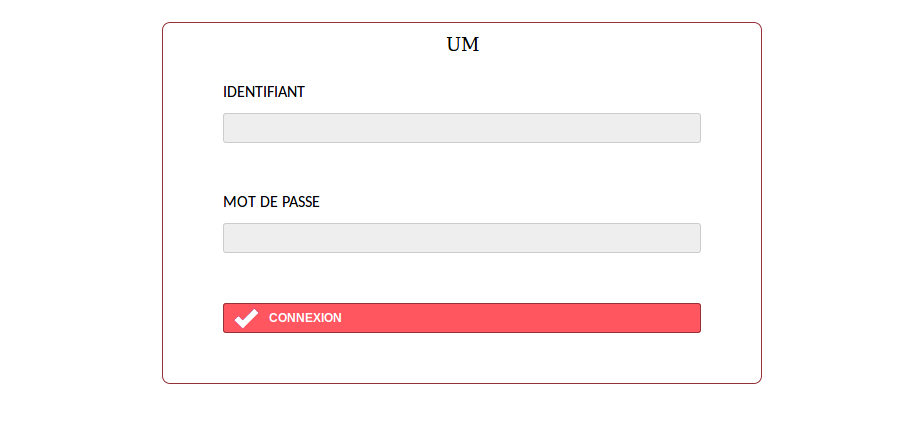
\includegraphics[width=19cm, center]{img/annexe/auth.png}
    \caption{Authentification} \medbreak
\end{figure}

\begin{figure}[H]
    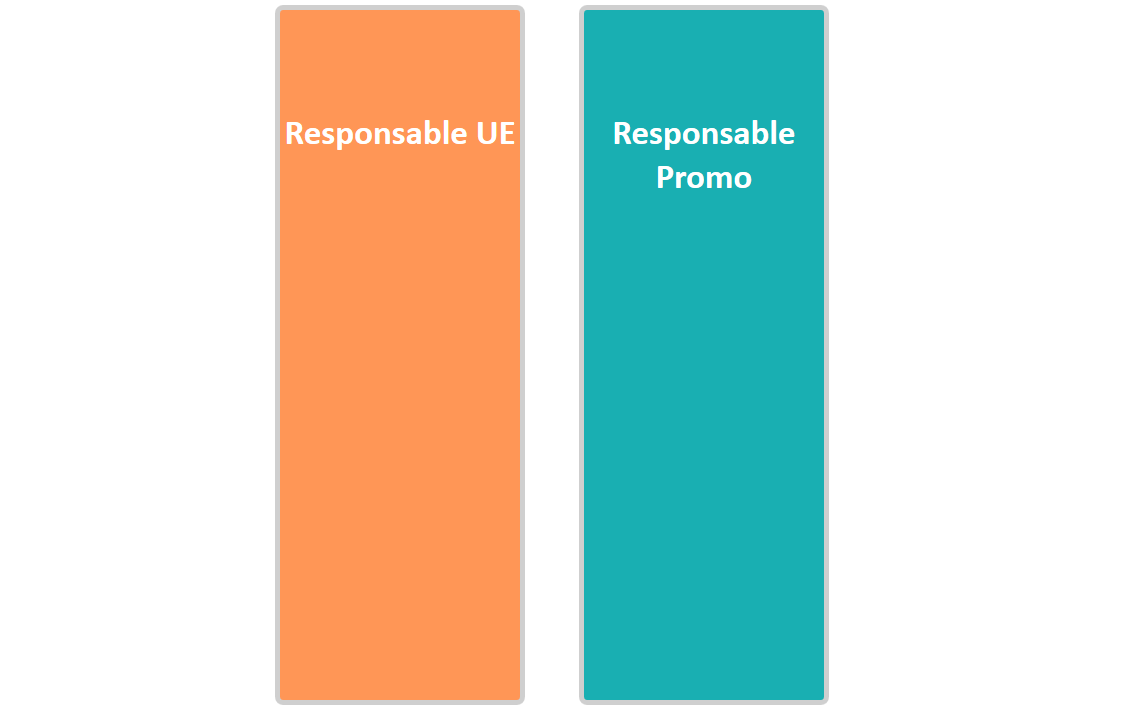
\includegraphics[width=19cm, center]{img/annexe/auth2.png}
    \caption{Choix de l'interface} \medbreak
\end{figure}

\begin{figure}[H]
    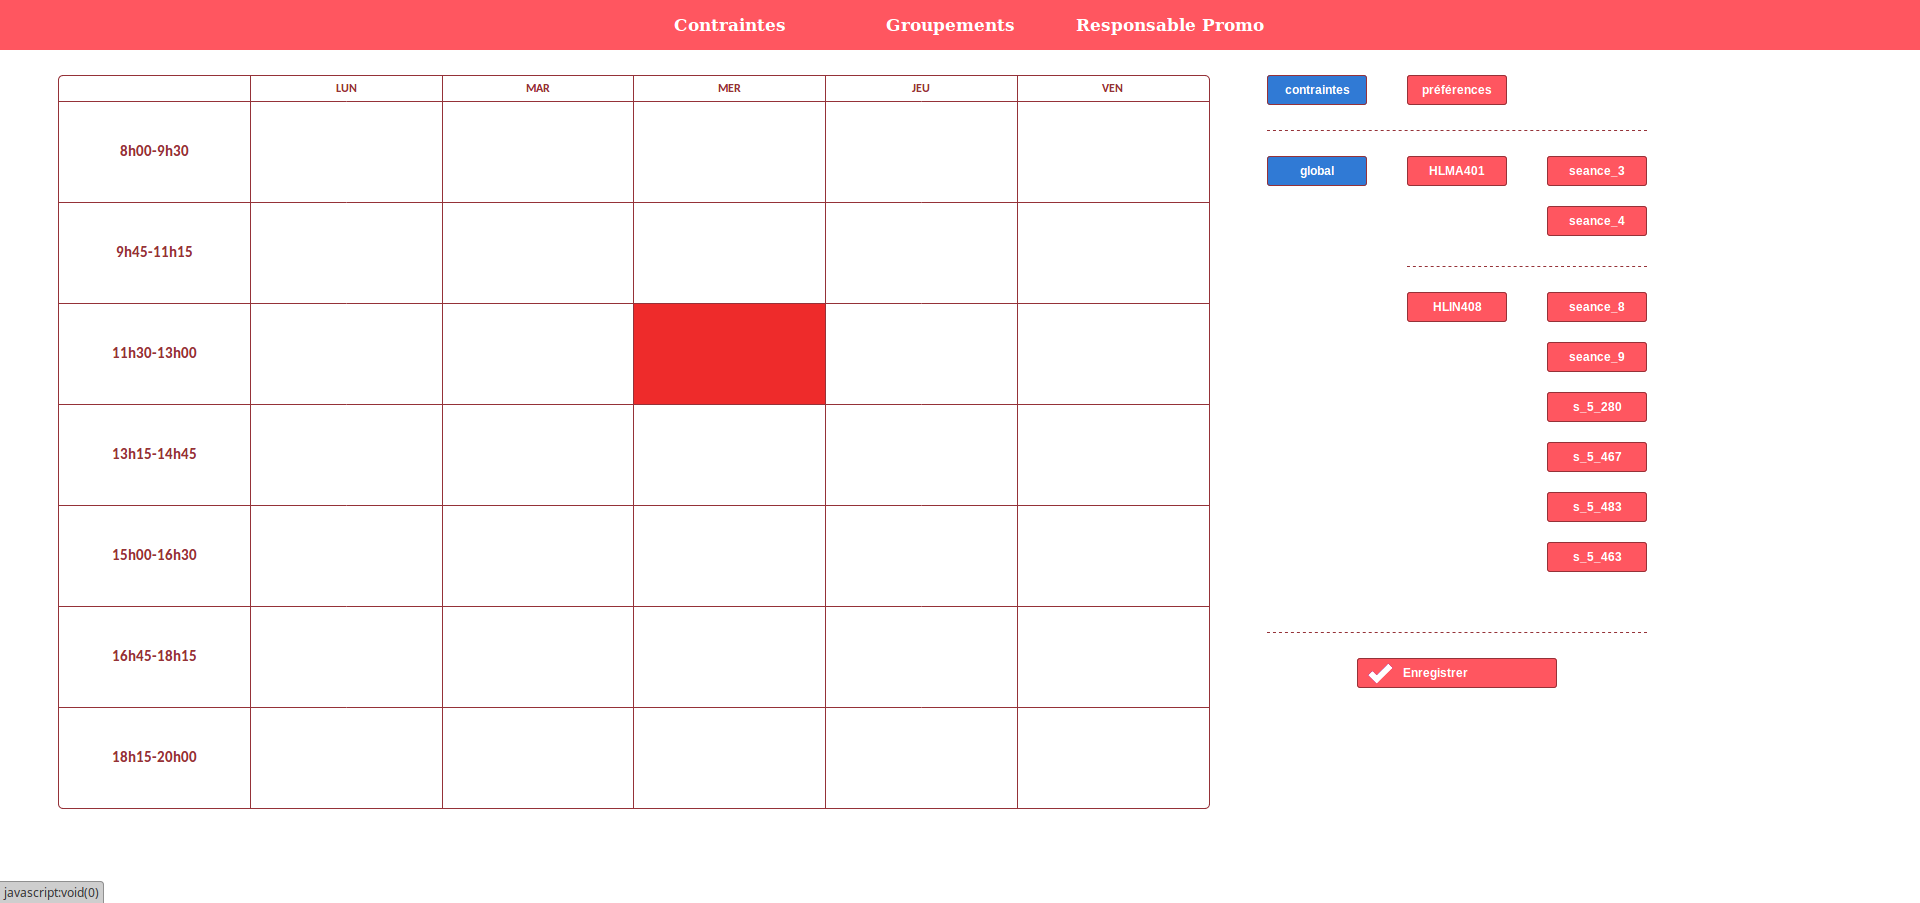
\includegraphics[width=19cm, center]{img/annexe/contrainte.png}
    \caption{Responsable d'UE : saisir des contraintes} \medbreak
\end{figure}

\begin{figure}[H]
    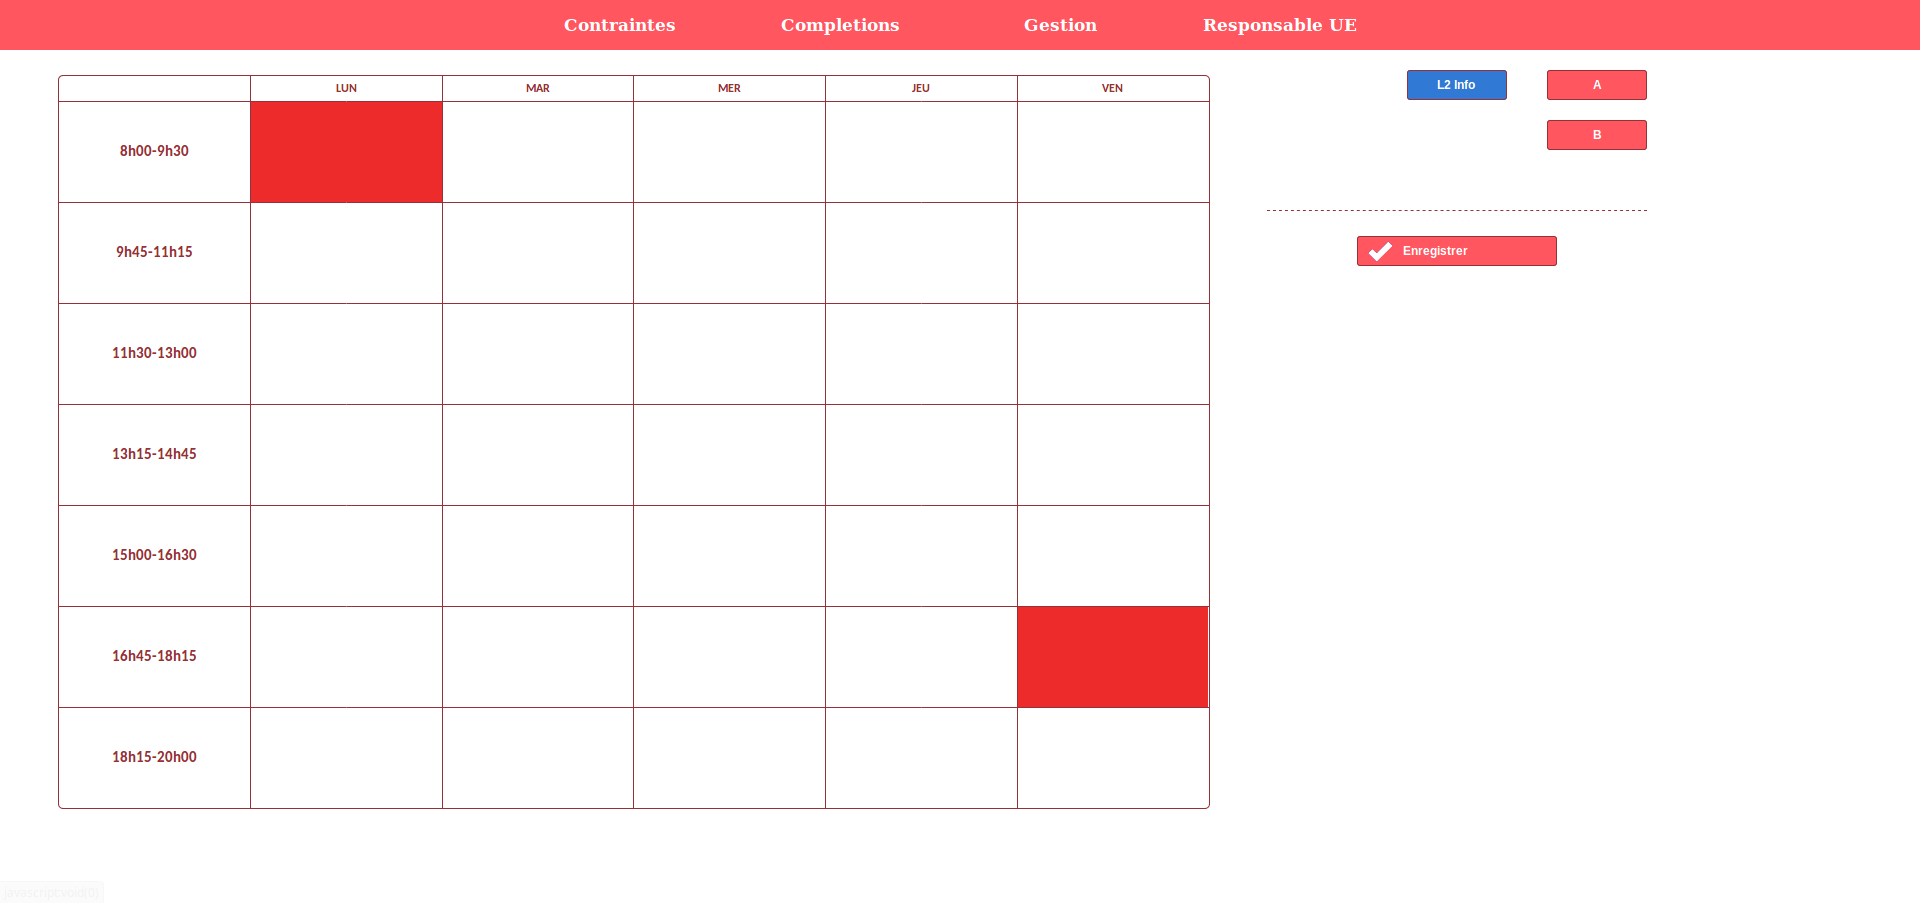
\includegraphics[width=19cm, center]{img/annexe/contrainte2.png}
    \caption{Responsable de promotion : saisir des contraintes} \medbreak
\end{figure}

\begin{figure}[H]
    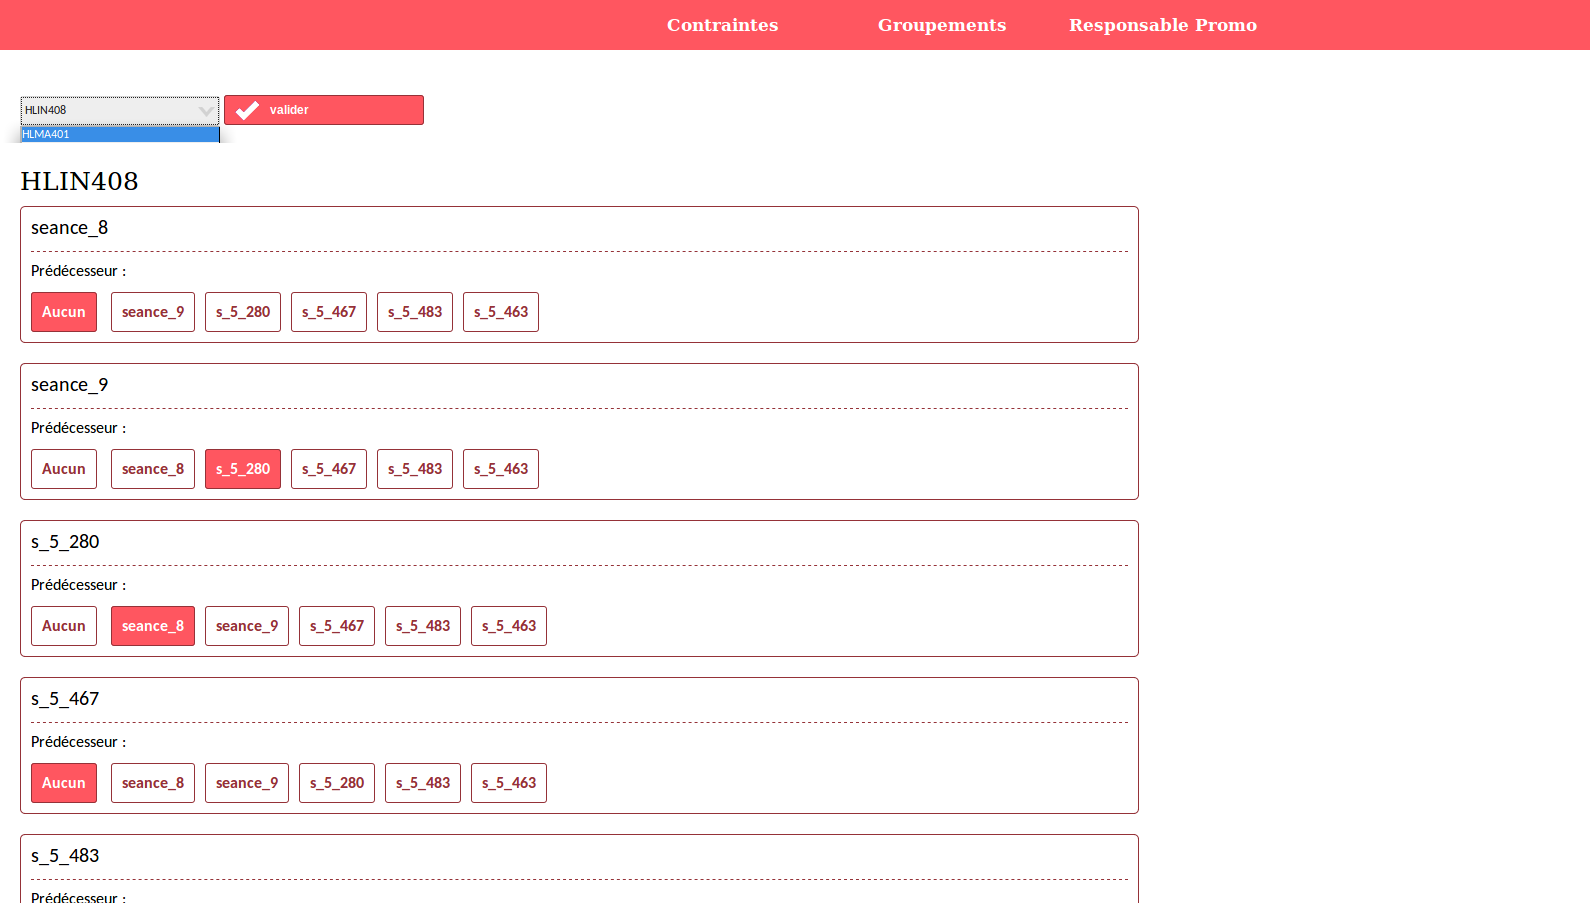
\includegraphics[width=19cm, center]{img/annexe/groupement.png}
    \caption{Enchainer des séances} \medbreak
\end{figure}

\begin{figure}[H]
    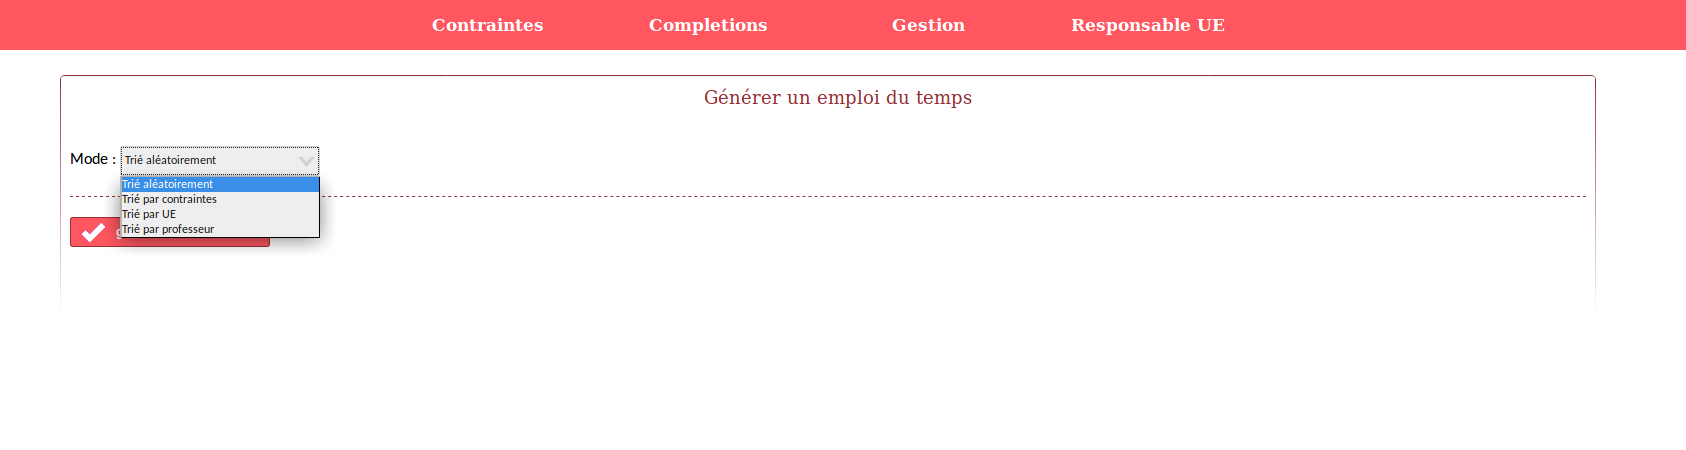
\includegraphics[width=19cm, center]{img/annexe/edt_pre.png}
    \caption{générer un emploi du temps} \medbreak
\end{figure}

\section{Exemple d'emploi du temps}
\begin{figure}[H]
    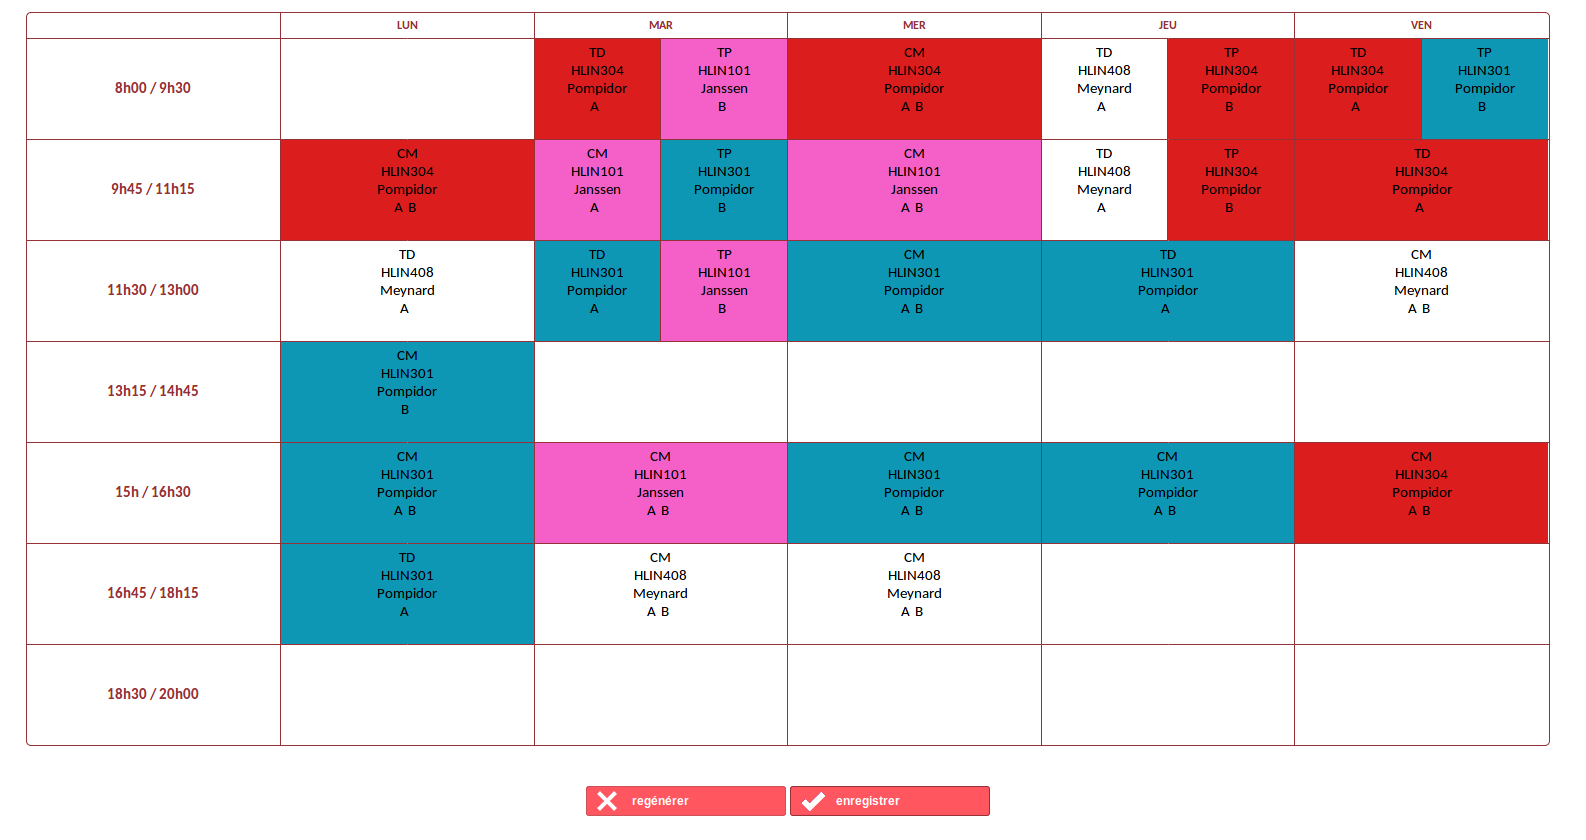
\includegraphics[width=19cm, center]{img/annexe/edt.png}
    \caption{Emploi du temps généré} \medbreak
\end{figure}

\end{document}
